\documentclass[10pt,a4paper,twocolumn]{article}
\usepackage[margin=1.8cm,columnsep=0.6cm]{geometry}
\usepackage[T1]{fontenc}
\usepackage{lmodern}
\usepackage{microtype}
\usepackage{amsmath}
\usepackage{booktabs}
\usepackage{graphicx}
\usepackage{xcolor}
\usepackage{tikz}
\usetikzlibrary{positioning,arrows.meta,fit}
\usepackage{caption}
\captionsetup{font=small,labelfont=bf}
\usepackage[numbers,sort&compress]{natbib}
\usepackage[colorlinks=true,linkcolor=black,citecolor=blue!50!black,urlcolor=blue!50!black]{hyperref}
\usepackage{url}
\usepackage{enumitem}
\setlist{nosep,leftmargin=*}

\newcommand{\AccPaperMaj}{20.1}
\newcommand{\FonePaperMaj}{4.8}
\newcommand{\FwPaperMaj}{6.8}
\newcommand{\AccPaperSvm}{77.1}
\newcommand{\FonePaperSvm}{76.7}
\newcommand{\FwPaperSvm}{76.9}
\newcommand{\AccPaperRf}{69.4}
\newcommand{\FonePaperRf}{68.0}
\newcommand{\FwPaperRf}{68.4}
\newcommand{\AccPaperCnn}{79.2}
\newcommand{\FonePaperCnn}{78.6}
\newcommand{\FwPaperCnn}{79.0}
\newcommand{\AccPaperLstm}{81.2}
\newcommand{\FonePaperLstm}{80.6}
\newcommand{\FwPaperLstm}{81.1}
\newcommand{\AccPaperEns}{81.9}
\newcommand{\FonePaperEns}{81.4}
\newcommand{\FwPaperEns}{81.9}
\newcommand{\AccLeakyMaj}{20.0}
\newcommand{\FoneLeakyMaj}{4.8}
\newcommand{\FwLeakyMaj}{6.6}
\newcommand{\AccLeakySvm}{85.6}
\newcommand{\FoneLeakySvm}{85.4}
\newcommand{\FwLeakySvm}{85.6}
\newcommand{\AccLeakyRf}{71.5}
\newcommand{\FoneLeakyRf}{70.5}
\newcommand{\FwLeakyRf}{70.7}
\newcommand{\AccLeakyCnn}{95.7}
\newcommand{\FoneLeakyCnn}{95.7}
\newcommand{\FwLeakyCnn}{95.6}
\newcommand{\AccLeakyLstm}{94.4}
\newcommand{\FoneLeakyLstm}{94.5}
\newcommand{\FwLeakyLstm}{94.4}
\newcommand{\AccLeakyEns}{96.5}
\newcommand{\FoneLeakyEns}{96.6}
\newcommand{\FwLeakyEns}{96.5}
\newcommand{\AccSpkMaj}{20.0}
\newcommand{\FoneSpkMaj}{4.8}
\newcommand{\FwSpkMaj}{6.7}
\newcommand{\AccStdSpkMaj}{0.0}
\newcommand{\AccSpkSvm}{49.1}
\newcommand{\FoneSpkSvm}{48.8}
\newcommand{\FwSpkSvm}{49.2}
\newcommand{\AccStdSpkSvm}{4.3}
\newcommand{\AccSpkRf}{46.8}
\newcommand{\FoneSpkRf}{43.3}
\newcommand{\FwSpkRf}{44.6}
\newcommand{\AccStdSpkRf}{2.6}
\newcommand{\AccSpkCnn}{56.7}
\newcommand{\FoneSpkCnn}{56.0}
\newcommand{\FwSpkCnn}{56.6}
\newcommand{\AccStdSpkCnn}{2.0}
\newcommand{\AccSpkLstm}{56.5}
\newcommand{\FoneSpkLstm}{56.2}
\newcommand{\FwSpkLstm}{56.4}
\newcommand{\AccStdSpkLstm}{2.9}
\newcommand{\AccSpkEns}{58.5}
\newcommand{\FoneSpkEns}{57.8}
\newcommand{\FwSpkEns}{58.2}
\newcommand{\AccStdSpkEns}{1.9}
\newcommand{\AccRTMaj}{14.3}
\newcommand{\FoneRTMaj}{3.6}
\newcommand{\FwRTMaj}{3.6}
\newcommand{\AccRTSvm}{23.9}
\newcommand{\FoneRTSvm}{17.2}
\newcommand{\FwRTSvm}{17.2}
\newcommand{\AccRTRf}{31.1}
\newcommand{\FoneRTRf}{23.8}
\newcommand{\FwRTRf}{23.8}
\newcommand{\AccRTCnn}{17.8}
\newcommand{\FoneRTCnn}{14.3}
\newcommand{\FwRTCnn}{14.3}
\newcommand{\AccRTLstm}{17.9}
\newcommand{\FoneRTLstm}{17.1}
\newcommand{\FwRTLstm}{17.1}
\newcommand{\AccRTEns}{19.7}
\newcommand{\FoneRTEns}{17.0}
\newcommand{\FwRTEns}{17.0}
\newcommand{\AccTRMaj}{20.0}
\newcommand{\FoneTRMaj}{4.8}
\newcommand{\FwTRMaj}{6.7}
\newcommand{\AccTRSvm}{13.6}
\newcommand{\FoneTRSvm}{7.7}
\newcommand{\FwTRSvm}{8.0}
\newcommand{\AccTRRf}{14.4}
\newcommand{\FoneTRRf}{5.6}
\newcommand{\FwTRRf}{5.2}
\newcommand{\AccTRCnn}{14.1}
\newcommand{\FoneTRCnn}{6.6}
\newcommand{\FwTRCnn}{6.2}
\newcommand{\AccTRLstm}{13.6}
\newcommand{\FoneTRLstm}{4.0}
\newcommand{\FwTRLstm}{3.7}
\newcommand{\AccTREns}{14.1}
\newcommand{\FoneTREns}{6.6}
\newcommand{\FwTREns}{6.2}
\newcommand{\LeakyAccNoise}{95.8}
\newcommand{\LeakyAccNoisepitch}{95.6}
\newcommand{\LeakyAccOriginal}{97.8}
\newcommand{\LeakyAccPitch}{97.1}
\newcommand{\LeakyOverlap}{99.1}
\newcommand{\GenderMaleSvm}{45.3}
\newcommand{\GenderFemaleSvm}{52.9}
\newcommand{\GenderGapSvm}{+7.6}
\newcommand{\GenderPSvm}{0.004}
\newcommand{\GenderMaleRf}{41.0}
\newcommand{\GenderFemaleRf}{52.6}
\newcommand{\GenderGapRf}{+11.7}
\newcommand{\GenderPRf}{$<$0.001}
\newcommand{\GenderMaleCnn}{49.4}
\newcommand{\GenderFemaleCnn}{63.9}
\newcommand{\GenderGapCnn}{+14.4}
\newcommand{\GenderPCnn}{$<$0.001}
\newcommand{\GenderMaleLstm}{47.2}
\newcommand{\GenderFemaleLstm}{65.8}
\newcommand{\GenderGapLstm}{+18.6}
\newcommand{\GenderPLstm}{$<$0.001}
\newcommand{\GenderMaleEns}{50.7}
\newcommand{\GenderFemaleEns}{66.2}
\newcommand{\GenderGapEns}{+15.6}
\newcommand{\GenderPEns}{$<$0.001}
\newcommand{\ActorAccMin}{40.0}
\newcommand{\ActorAccMax}{81.7}
\newcommand{\ActorMin}{Actor~09}
\newcommand{\ActorMax}{Actor~08}
\newcommand{\GenderActorU}{129}
\newcommand{\GenderActorP}{0.001}
\newcommand{\ConfOne}{sad$\to$neutral}
\newcommand{\ConfOnePct}{27.6}
\newcommand{\ConfTwo}{neutral$\to$sad}
\newcommand{\ConfTwoPct}{13.5}
\newcommand{\ConfThree}{happy$\to$fearful}
\newcommand{\ConfThreePct}{13.5}
\newcommand{\SpkRecallMin}{34.4}
\newcommand{\SpkRecallMinName}{sad}
\newcommand{\SpkRecallMax}{73.4}
\newcommand{\SpkRecallMaxName}{angry}
\newcommand{\TessAccOaf}{15.5}
\newcommand{\TessAccYaf}{23.9}
\newcommand{\TessTopPred}{sad}
\newcommand{\TessTopPredShare}{53.1}
\newcommand{\OffsetAccPaper}{19.7}
\newcommand{\OffsetAccZero}{30.5}
\newcommand{\OffsetFoneZero}{28.2}
\newcommand{\OffsetPadPaper}{42}
\newcommand{\OffsetPadZero}{18}
\newcommand{\OffsetSadPaper}{53}
\newcommand{\OffsetSadZero}{11}
\newcommand{\RavTopPred}{fearful}
\newcommand{\RavTopPredShare}{87.9}
\newcommand{\FitMinMaj}{0.0}
\newcommand{\InferMsMaj}{0.00}
\newcommand{\FitMinSvm}{0.1}
\newcommand{\InferMsSvm}{0.26}
\newcommand{\FitMinRf}{0.0}
\newcommand{\InferMsRf}{0.67}
\newcommand{\ParamsCnn}{616{,}615}
\newcommand{\FitMinCnn}{10.6}
\newcommand{\InferMsCnn}{2.70}
\newcommand{\EpochsCnn}{21}
\newcommand{\ParamsLstm}{688{,}807}
\newcommand{\FitMinLstm}{13.1}
\newcommand{\InferMsLstm}{4.14}
\newcommand{\EpochsLstm}{23}
\newcommand{\ParamsEns}{1{,}305{,}422}
\newcommand{\LeakGainEns}{14.6}
\newcommand{\LeakGainSvm}{8.5}
\newcommand{\ReportedGapEns}{15.6}
\newcommand{\SpkDropEns}{23.5}
\newcommand{\SpkEnsOverSvm}{9.4}
\newcommand{\PaperEnsOverSvm}{4.9}
\newcommand{\OffsetGain}{10.8}
\newcommand{\NumTrainings}{16}
\newcommand{\ComputeHours}{3}
\newcommand{\TessPadPct}{42}
\newcommand{\RavPadPct}{0}


\title{\textbf{How Far Does a Near-Perfect Speech Emotion Recogniser Generalise?}\\[2pt]
\large Replication and Stress-Testing of a Lightweight Hand-Crafted-Feature Ensemble}
\author{Group F26-11 \quad 22L-7786 (Lead) \quad 23L-3002\\
\small AI2002 Artificial Intelligence (BS-SE-5A), FAST-NUCES Lahore, Fall 2026 --- Track B (R\&D)\\
\small Instructor: Hajra Waheed \quad TA: Muhammad Abdullah Shahid}
\date{}

\begin{document}
\maketitle

\begin{abstract}
Chowdhury et al.\ (\emph{Scientific Reports}, 2025) report 97.57\% accuracy on RAVDESS and 100\% on TESS for a
lightweight averaging ensemble of a 1D-CNN and a CNN\_Bi-LSTM trained on hand-crafted features (ZCR, RMSE, MFCC,
Chroma STFT). We re-implement the pipeline from the paper's specification and stress-test it with four evaluation
protocols, classical baselines, a gender-bias check and a feature ablation. With augmentation applied only to
training clips, the ensemble reaches \AccPaperEns\%; applying augmentation \emph{before} the train--test split, so that
\LeakyOverlap\% of test samples have an augmented copy in training, reproduces the paper's level (\AccLeakyEns\%).
For speakers never seen in training, accuracy falls to \AccSpkEns\,$\pm$\,\AccStdSpkEns\%, and across corpora it is
near chance (\AccRTEns\% RAVDESS$\to$TESS, \AccTREns\% TESS$\to$RAVDESS). All models are significantly more accurate
for female than male actors (ensemble \GenderFemaleEns\% vs.\ \GenderMaleEns\%, $p<0.001$; actor-level
$p=\GenderActorP$). The architecture is a sound lightweight model, but its headline accuracy depends on the
evaluation protocol; speaker-independent and cross-corpus evaluation should be the standard for reporting SER results.
\end{abstract}

\section{Introduction}
Speech emotion recognition (SER) classifies a speaker's emotional state from the voice alone and is used in
call-centre analytics, health screening and conversational agents. Chowdhury et al.~\cite{chowdhury2025}
recently showed that a \emph{lightweight} ensemble of a 1D-CNN and a CNN\_Bi-LSTM, trained on four classical
hand-crafted features (ZCR, RMSE, MFCC and Chroma STFT), reaches 97.57\% accuracy on RAVDESS and 100\% on TESS,
outperforming heavier spectrogram-based models. Such numbers are attractive for low-resource deployment, but they
were obtained by training and testing on random splits of the \emph{same} dataset, the paper does not state whether
augmentation was applied before or after splitting, and the authors themselves list cross-dataset validation as
future work~\cite[Sec.~7]{chowdhury2025}.

\paragraph{Research question.} \emph{Does the near-perfect accuracy of this lightweight model reflect emotion
recognition that transfers to new clips, new speakers and new recording conditions, and is it equally accurate for
male and female speakers?} We re-implement the full pipeline from the paper's specification and test six hypotheses:
\begin{enumerate}[label=\textbf{H\arabic*}]
  \item \textbf{Replication:} under the paper's protocol our implementation approaches the reported RAVDESS accuracy.
  \item \textbf{Split order:} augmenting \emph{before} splitting inflates accuracy, because augmented copies of a
        test clip then appear in training.
  \item \textbf{Unseen speakers:} accuracy drops substantially when test actors are never seen in training.
  \item \textbf{Unseen dataset:} accuracy collapses when training on RAVDESS and testing on TESS (and vice versa).
  \item \textbf{Gender bias:} speaker-independent accuracy differs between male and female actors.
  \item \textbf{Features:} MFCC carries most of the information; Chroma adds a smaller but positive contribution,
        as the paper's LIME analysis suggests.
\end{enumerate}

\paragraph{Contributions.} (i) An open, reproducible re-implementation of the paper's features, augmentation,
architectures and training schedule; (ii) a controlled comparison of four evaluation protocols of increasing
strictness, with classical baselines; (iii) the gender-bias check required by the course; (iv) a feature and
augmentation ablation; (v) an error analysis explaining \emph{why} performance changes between protocols.

\section{Data}
We use the two Kaggle datasets used by the paper~\cite{kaggleravdess,kaggletess}.
\textbf{RAVDESS}~\cite{livingstone2018}: 1,440 speech clips (16-bit, 48\,kHz) from 24 professional actors
(12 male, 12 female, odd IDs male) speaking two fixed sentences in eight emotions at two intensities.
\textbf{TESS}~\cite{tess2020}: 2,800 clips (24.4\,kHz) of the carrier phrase ``Say the word \_\_'' with 200 target
words, spoken by two female actors aged 26 (YAF) and 64 (OAF) in seven emotions. Both Kaggle copies contain
duplicated folders; our loader de-duplicates by filename to avoid train--test overlap.

Following the paper's Table~1 (288 neutral RAVDESS clips), RAVDESS \emph{calm} is merged into \emph{neutral}, and TESS
\emph{pleasant surprise} is mapped to \emph{surprised}, giving one 7-class label set for both corpora:
neutral, happy, sad, angry, fearful, disgust, surprised. RAVDESS is balanced except neutral (288 vs.\ 192 per class);
TESS is perfectly balanced (400 per class).

\section{Methodology}
\begin{figure*}[t]
\centering
\resizebox{\textwidth}{!}{%
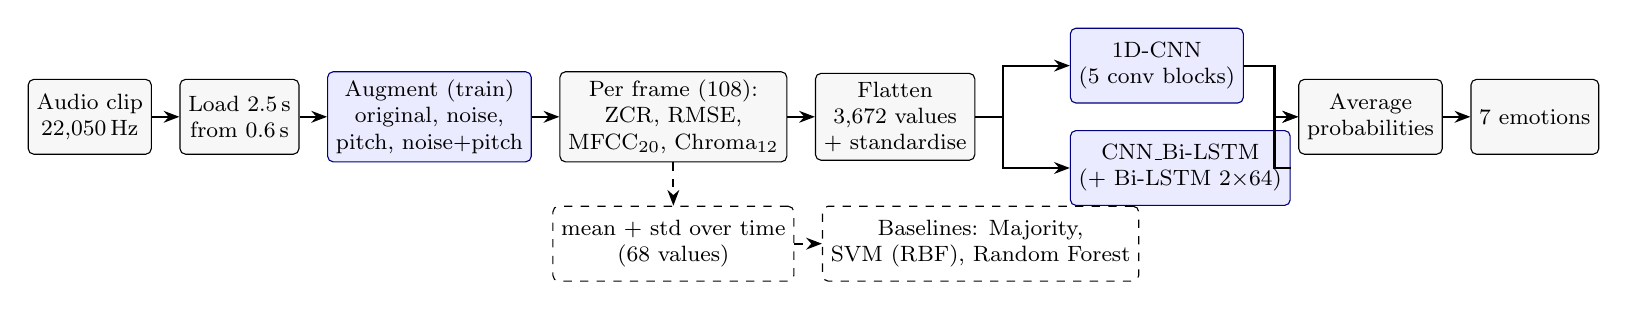
\begin{tikzpicture}[node distance=0.35cm, font=\footnotesize,
  box/.style={draw, rounded corners=2pt, align=center, minimum height=0.95cm, inner sep=3pt, fill=gray!6},
  hl/.style={box, fill=blue!8, draw=blue!50!black},
  arr/.style={-{Stealth[length=2mm]}, thick}]
\node[box] (wav) {Audio clip\\22{,}050\,Hz};
\node[box, right=of wav] (crop) {Load 2.5\,s\\from 0.6\,s};
\node[hl, right=of crop] (aug) {Augment (train)\\original, noise,\\pitch, noise+pitch};
\node[box, right=of aug] (feat) {Per frame (108):\\ZCR, RMSE,\\MFCC$_{20}$, Chroma$_{12}$};
\node[box, right=of feat] (flat) {Flatten\\3{,}672 values\\+ standardise};
\node[hl, right=1.2cm of flat, yshift=0.65cm] (cnn) {1D-CNN\\(5 conv blocks)};
\node[hl, right=1.2cm of flat, yshift=-0.65cm] (lstm) {CNN\_Bi-LSTM\\(+ Bi-LSTM 2$\times$64)};
\node[box, right=0.9cm of flat, xshift=3.2cm] (avg) {Average\\probabilities};
\node[box, right=of avg] (out) {7 emotions};
\draw[arr] (wav) -- (crop); \draw[arr] (crop) -- (aug); \draw[arr] (aug) -- (feat); \draw[arr] (feat) -- (flat);
\draw[arr] (flat.east) -- ++(0.35,0) |- (cnn.west); \draw[arr] (flat.east) -- ++(0.35,0) |- (lstm.west);
\draw[arr] (cnn.east) -| ([xshift=-0.3cm]avg.west) -- (avg.west); \draw[arr] (lstm.east) -| ([xshift=-0.3cm]avg.west) -- (avg.west);
\draw[arr] (avg) -- (out);
\node[box, below=0.55cm of feat, fill=white, dashed] (pool) {mean + std over time\\(68 values)};
\node[box, right=of pool, fill=white, dashed] (base) {Baselines: Majority,\\SVM (RBF), Random Forest};
\draw[arr, dashed] (feat) -- (pool); \draw[arr, dashed] (pool) -- (base);
\end{tikzpicture}}
\caption{Pipeline. Blue boxes follow the paper~\cite{chowdhury2025}; dashed boxes are our classical baselines, which use
the same frame features summarised over time.}
\label{fig:pipeline}
\end{figure*}

\subsection{Features and augmentation}
All settings follow the paper's Section~4 (Fig.~\ref{fig:pipeline}). Audio is resampled to 22,050\,Hz and 2.5\,s are
loaded from an offset of 0.6\,s. With a 2,048-sample frame and 512-sample hop this gives 108 frames. Per frame we
compute ZCR (1), RMSE (1), 20 MFCCs and 12 Chroma STFT bins (librosa~\cite{mcfee2015librosa}); clips shorter than
2.5\,s are zero-filled, as in the paper (``null values were replaced with zeroes''). Features are flattened and
concatenated into the paper's 3,672-dimensional vector ($108 \times 34$) and standardised per dimension with
training-set statistics. Each training clip contributes four versions, exactly as in the paper: the original,
Gaussian noise with amplitude $\alpha\!=\!0.035\cdot u\cdot\max|x|$ ($u\sim U(0,1)$), a pitch shift of 0.7
semitones, and noise followed by pitch shift. Validation and test clips are never augmented, except in the
deliberately leaky protocol below.

\subsection{Models}
\textbf{Paper models.} We implement the paper's Table~2 architecture in Keras~\cite{abadi2015tensorflow}: five
convolution blocks (Conv1D $\to$ BatchNorm $\to$ MaxPool/2) with 128, 128, 64, 64 and 32 filters, kernel sizes 5, 5,
5, 3, 3, ReLU, ``same'' padding, and 20\% dropout after blocks 2, 4 and 5; then Flatten, Dense(128, ReLU),
BatchNorm and a 7-way softmax. CNN\_Bi-LSTM inserts a bidirectional LSTM (64 units per direction, full sequence)
before block 5. The \textbf{averaging ensemble} is the mean of the two models' class probabilities, which is what
the paper's Average layer computes at inference. Our CNN\_Bi-LSTM has \ParamsLstm{} parameters versus 672,423 in the
paper's Table~2; the small difference comes from the last convolution, whose parameter count in the paper
(6,176) implies 64 input channels although the Bi-LSTM listed before it outputs 128.

\textbf{Training (paper Table~3).} Adam (learning rate $10^{-3}$), cross-entropy, batch size 64, up to 100 epochs,
early stopping on validation accuracy (patience 5, best weights restored), and learning-rate halving on a
validation-accuracy plateau (patience 3, minimum $10^{-5}$). All random seeds are fixed to 42.

\textbf{Baselines} (scikit-learn~\cite{pedregosa2011sklearn}) use the mean and standard deviation of each frame
feature over time (68 values): a majority-class predictor (chance level), an RBF SVM ($C\!=\!10$) and a 300-tree
Random Forest. They are trained on exactly the same (augmented) training clips as the deep models.

\subsection{Evaluation protocols}
\begin{enumerate}[label=\textbf{P\arabic*}]
  \item \textbf{Paper protocol} (H1): stratified random 80/10/10 split of the 1,440 RAVDESS clips;
        augmentation applied to the 1,152 training clips only (4,608 training samples, as in the paper).
  \item \textbf{Augment-before-split} (H2): all 5,760 augmented samples are pooled and then split 80/10/10 at random,
        so a test clip's augmented copies can be in the training set.
  \item \textbf{Speaker-independent} (H3, H5): 4-fold cross-validation in which each fold holds out six
        actors (three male, three female): actors 1--6, 7--12, 13--18, 19--24. Every clip is tested exactly once
        by a model that never heard that speaker; 10\% of the training clips are held out for early stopping.
  \item \textbf{Cross-dataset} (H4): train on all of RAVDESS and test on all of TESS, and the reverse. No target
        data is used for training, early stopping or normalisation.
\end{enumerate}
The ablation (H6) retrains the 1D-CNN and SVM under P1 with one feature group removed, with MFCC only, and
without augmentation. We report accuracy, macro-F1 (robust to RAVDESS's larger neutral class) and, for comparison
with the paper, weighted F1. The \textbf{bias check} compares accuracy on the 12 male versus the 12 female RAVDESS
actors under P3 with a two-proportion $z$-test ($n\!=\!720$ clips per group).

\section{Results}
Table~\ref{tab:main} summarises all models under the four protocols; Fig.~\ref{fig:comparison} visualises the three
RAVDESS-based protocols and the RAVDESS$\to$TESS transfer.

\begin{table*}[t]
\centering
\caption{Accuracy / macro-F1 (\%) on the test sets. Speaker-independent: pooled over all 1,440 clips, $\pm$ is the
standard deviation of accuracy across the 4 speaker folds. Chance (majority class) is 20.0\% on RAVDESS and 14.3\% on
TESS. Bold: best model per protocol, when above chance.}
\label{tab:main}
\begin{tabular}{lccccc}
\toprule
Model & Paper protocol & Aug.-before-split & Speaker-indep. & RAV$\to$TESS & TESS$\to$RAV \\
\midrule
Majority class & 20.1 / 4.8 & 20.0 / 4.8 & 20.0\,$\pm$\,0.0 / 4.8 & 14.3 / 3.6 & 20.0 / 4.8 \\
SVM (RBF) & 77.1 / 76.7 & 85.6 / 85.4 & 49.1\,$\pm$\,4.3 / 48.8 & 23.9 / 17.2 & 13.6 / 7.7 \\
Random Forest & 69.4 / 68.0 & 71.5 / 70.5 & 46.8\,$\pm$\,2.6 / 43.3 & \textbf{31.1 / 23.8} & 14.4 / 5.6 \\
\midrule
1D-CNN & 79.2 / 78.6 & 95.7 / 95.7 & 56.7\,$\pm$\,2.0 / 56.0 & 17.8 / 14.3 & 14.1 / 6.6 \\
CNN\_Bi-LSTM & 81.2 / 80.6 & 94.4 / 94.5 & 56.5\,$\pm$\,2.9 / 56.2 & 17.9 / 17.1 & 13.6 / 4.0 \\
Averaging ensemble & \textbf{81.9 / 81.4} & \textbf{96.5 / 96.6} & \textbf{58.5\,$\pm$\,1.9 / 57.8} & 19.7 / 17.0 & 14.1 / 6.6 \\
\bottomrule
\end{tabular}

\end{table*}

\begin{figure*}[t]
\centering
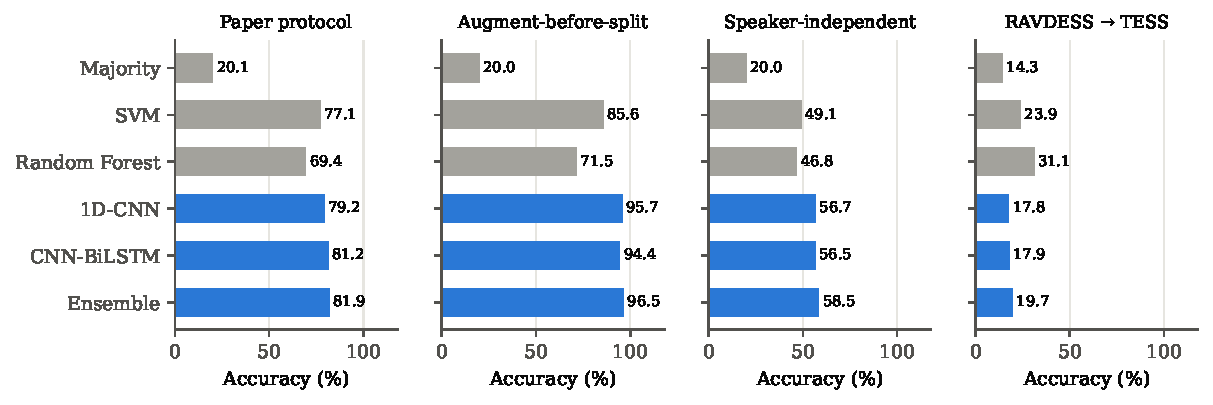
\includegraphics[width=\textwidth]{../results/figures/fig_model_comparison.pdf}
\caption{Accuracy of every model as the protocol becomes stricter (left to right). Grey: classical baselines;
blue: the paper's models. The same ensemble ranges from \AccLeakyEns\% to \AccRTEns\%.}
\label{fig:comparison}
\end{figure*}

\subsection{H1 -- Replication under the paper's protocol}
With augmentation applied to training clips only, our ensemble reaches \AccPaperEns\% accuracy
(weighted F1 \FwPaperEns\%), \ReportedGapEns{} points below the 97.57\% reported (Table~\ref{tab:replication}). The ordering of the
models matches the paper (ensemble $\geq$ CNN\_Bi-LSTM $\geq$ 1D-CNN), and all deep models beat the SVM
(\AccPaperSvm\%) and Random Forest (\AccPaperRf\%). \textbf{H1 is not supported}: the reported figure is not
reproduced under a leak-free split.

\begin{table}[t]
\centering
\caption{RAVDESS replication: accuracy and weighted F1 (\%).}
\label{tab:replication}
\footnotesize\setlength{\tabcolsep}{3pt}
\resizebox{\columnwidth}{!}{\begin{tabular}{lcccccc}
\toprule
 & \multicolumn{2}{c}{Reported in paper} & \multicolumn{2}{c}{Ours: paper protocol} & \multicolumn{2}{c}{Ours: aug.-before-split} \\
\cmidrule(lr){2-3}\cmidrule(lr){4-5}\cmidrule(lr){6-7}
Model & Acc. & W-F1 & Acc. & W-F1 & Acc. & W-F1 \\
\midrule
1D-CNN & 96.18 & 96.22 & 79.17 & 79.04 & 95.66 & 95.65 \\
CNN\_Bi-LSTM & 97.57 & 97.29 & 81.25 & 81.14 & 94.44 & 94.44 \\
Averaging ensemble & 97.57 & 97.56 & 81.94 & 81.94 & 96.53 & 96.53 \\
\bottomrule
\end{tabular}
}
\end{table}

\subsection{H2 -- Augmenting before splitting inflates accuracy}
When the 5,760 augmented samples are pooled \emph{before} the 80/10/10 split, \LeakyOverlap\% of the test samples
have at least one augmented copy of the same recording in the training set. The ensemble then scores
\AccLeakyEns\% (1D-CNN \AccLeakyCnn\%), within about one percentage point of the paper's 97.57\% and 96.18\%.
Accuracy is \LeakyAccOriginal\% on original test clips and \LeakyAccNoisepitch\% on noise+pitch copies, i.e.\ the
model recognises recordings it has effectively already seen. \textbf{H2 is supported}. The paper does not state
the split order, so we cannot prove this is what happened there, but it is the only one of our settings that
reproduces its numbers, and the inflation (+\LeakGainEns{} points for the ensemble) is much larger for the high-capacity deep
models than for the SVM (+\LeakGainSvm), consistent with memorisation of near-duplicates~\cite{kapoor2023leakage}.

\subsection{H3 -- Unseen speakers}
Holding out whole actors lowers ensemble accuracy to \AccSpkEns\,$\pm$\,\AccStdSpkEns\% (macro-F1 \FoneSpkEns\%), a
drop of \SpkDropEns{} points from the paper protocol. The deep models still beat the best classical baseline
(SVM, \AccSpkSvm\%) by \SpkEnsOverSvm{} points, so they do learn transferable cues, but performance varies strongly between
speakers: from \ActorAccMin\% (\ActorMin) to \ActorAccMax\% (\ActorMax). Recall is highest for \SpkRecallMaxName{}
(\SpkRecallMax\%) and lowest for \SpkRecallMinName{} (\SpkRecallMin\%); the most frequent errors are
\ConfOne{} (\ConfOnePct\% of sad clips), \ConfTwo{} (\ConfTwoPct\%) and \ConfThree{} (\ConfThreePct\%)
(Fig.~\ref{fig:confusion}). \textbf{H3 is supported}.

\begin{figure*}[t]
\centering
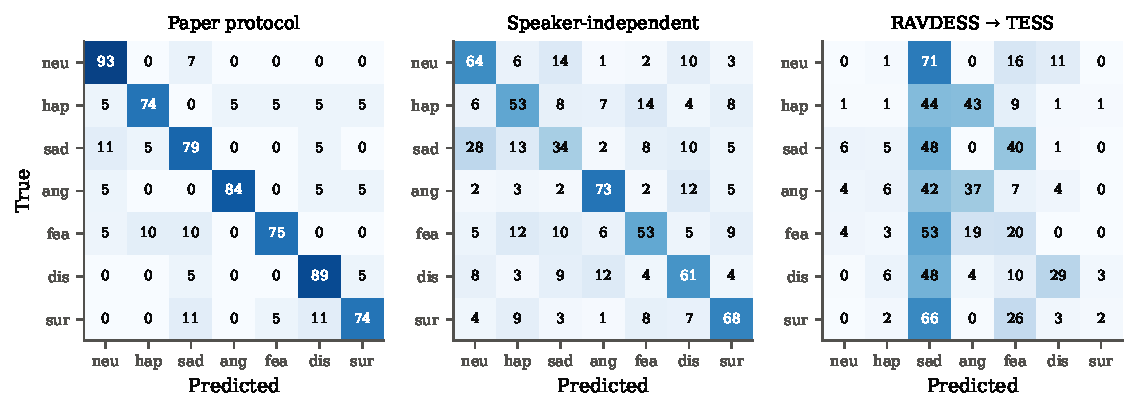
\includegraphics[width=0.92\textwidth]{../results/figures/fig_confusion.pdf}
\caption{Row-normalised confusion matrices (\%) of the ensemble. Under the paper protocol most mass is on the
diagonal; for unseen speakers low-arousal emotions (neutral, sad) are confused; on TESS predictions collapse onto a
few classes.}
\label{fig:confusion}
\end{figure*}

\subsection{H4 -- Unseen dataset}
Cross-corpus transfer fails in both directions. Trained on RAVDESS, the ensemble reaches only \AccRTEns\% on TESS
(chance 14.3\%) and labels \TessTopPredShare\% of all TESS clips as \emph{\TessTopPred}. Trained on TESS, it scores
\AccTREns\% on RAVDESS, \emph{below} the 20.0\% majority baseline, and predicts \emph{\RavTopPred} for
\RavTopPredShare\% of clips. Per-class recall on TESS (RAVDESS-trained ensemble) is:

\smallskip
\centerline{\small\begin{tabular}{ccccccc}
\toprule
Ang. & Dis. & Fea. & Hap. & Neu. & Sad. & Sur. \\
\midrule
37.0 & 29.2 & 20.2 & 0.8 & 0.2 & 48.5 & 2.0 \\
\bottomrule
\end{tabular}
}
\smallskip

\noindent Interestingly, the Random Forest transfers best (\AccRTRf\%). Its time-pooled statistics do not depend
on \emph{where} in the 2.5\,s window a sound occurs, whereas the paper's flattened vector ties every value to a
fixed frame position. \textbf{H4 is supported.}

\paragraph{Controlled check: zero padding.} TESS clips are short, so after the 0.6\,s offset \OffsetPadPaper\% of
TESS frames are zero padding, against \RavPadPct\% for RAVDESS. Silent frames have near-zero energy and look like
low-arousal speech. To test this without retraining, we re-extracted TESS with offset 0\,s
(\OffsetPadZero\% padding) and evaluated the \emph{same} RAVDESS-trained models: accuracy rises from
\OffsetAccPaper\% to \OffsetAccZero\% and the share of ``sad'' predictions falls from \OffsetSadPaper\% to
\OffsetSadZero\%. Padding therefore explains part of the collapse, but even without it the model remains far below
its within-corpus accuracy, pointing to the other differences between corpora: speakers, single words vs.\
sentences, and recording conditions. The older TESS speaker is recognised worse (\TessAccOaf\% vs.\
\TessAccYaf\% for the younger one).

\subsection{H5 -- Gender bias check}
Every model is more accurate for female than for male actors (Table~\ref{tab:gender}, Fig.~\ref{fig:gender}). For
the ensemble the gap is \GenderGapEns{} points (\GenderFemaleEns\% vs.\ \GenderMaleEns\%, $p$\,\GenderPEns{} by a
two-proportion $z$-test). Because clips of the same actor are not independent, we also compared the 24 per-actor
accuracies: the female actors are still clearly better (Mann--Whitney $U=\GenderActorU$ of a maximum 144,
$p=\GenderActorP$). The data are balanced (12 actors and 720 clips per gender), so this is not a sampling artefact
of RAVDESS's composition. The gap is largest for surprised, neutral and disgust and is the only one reversed for
happy (Table~\ref{tab:gender_emotion}). \textbf{H5 is supported}: a model deployed from this pipeline would
systematically serve male speakers worse.

\begin{table}[t]
\centering
\caption{Bias check, speaker-independent protocol (720 clips per gender). Gap = female $-$ male.}
\label{tab:gender}
\footnotesize\setlength{\tabcolsep}{3pt}
\resizebox{\columnwidth}{!}{\begin{tabular}{lccccc}
\toprule
Model & Acc. male & Acc. female & Gap (pp) & $z$ & $p$ \\
\midrule
SVM (RBF) & 45.3 & 52.9 & +7.6 & -2.90 & 0.004 \\
Random Forest & 41.0 & 52.6 & +11.7 & -4.44 & $<$0.001 \\
1D-CNN & 49.4 & 63.9 & +14.4 & -5.53 & $<$0.001 \\
CNN\_Bi-LSTM & 47.2 & 65.8 & +18.6 & -7.12 & $<$0.001 \\
Averaging ensemble & 50.7 & 66.2 & +15.6 & -5.99 & $<$0.001 \\
\bottomrule
\end{tabular}
}
\end{table}

\begin{figure}[t]
\centering
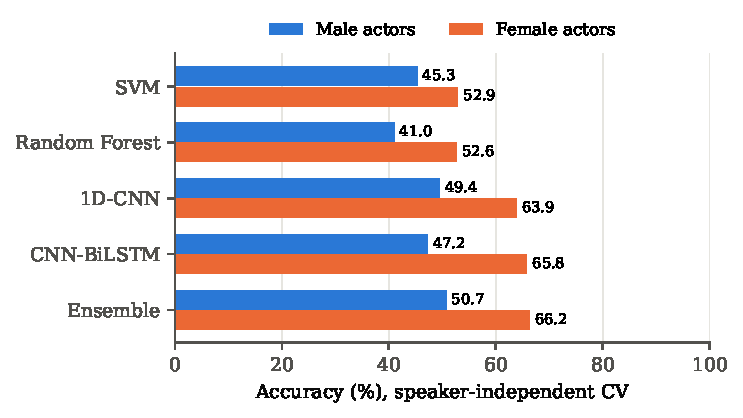
\includegraphics[width=\columnwidth]{../results/figures/fig_gender_bias.pdf}
\caption{Accuracy by speaker gender (speaker-independent CV).}
\label{fig:gender}
\end{figure}

\begin{table}[t]
\centering
\caption{Per-emotion recall (\%) of the ensemble by gender.}
\label{tab:gender_emotion}
\small
\begin{tabular}{lccc}
\toprule
Emotion & Recall male & Recall female & Gap (pp) \\
\midrule
Neutral & 54.2 & 74.3 & +20.1 \\
Happy & 54.2 & 52.1 & -2.1 \\
Sad & 30.2 & 38.5 & +8.3 \\
Angry & 67.7 & 79.2 & +11.5 \\
Fearful & 43.8 & 61.5 & +17.7 \\
Disgust & 51.0 & 70.8 & +19.8 \\
Surprised & 52.1 & 83.3 & +31.2 \\
\bottomrule
\end{tabular}

\end{table}

\subsection{H6 -- Feature and augmentation ablation}
\label{sec:ablation}
Table~\ref{tab:ablation} retrains the 1D-CNN and the SVM on the paper-protocol split with parts of the input removed.
The test set has 144 clips, so one clip is \AblClipPct{} points and the standard error of an accuracy near 79\%
is about \AblSE{} points; differences smaller than roughly twice that are not meaningful.

\begin{table}[t]
\centering
\caption{Ablation on the paper-protocol split (accuracy \%, 144 test clips). $\Delta$ is relative to the full
1D-CNN (79.2\%). *Training stopped at epoch 9 with validation accuracy at chance level (see text).}
\label{tab:ablation}
\footnotesize\setlength{\tabcolsep}{3pt}
\resizebox{\columnwidth}{!}{\input{generated/tab_ablation.tex}}
\end{table}

\begin{itemize}
  \item \textbf{MFCC is essential.} Removing the 20 MFCCs changes accuracy by \AblNomfcc{} points for the 1D-CNN and
        \AblSvmNomfcc{} for the SVM, the only feature removal clearly beyond noise. \emph{MFCC alone}
        (\AblAccMfcconly\%) is at least as accurate as the full feature set.
  \item \textbf{ZCR and RMSE add nothing measurable} ($\Delta$ of \AblNozcr{} and \AblNorms{} points).
  \item \textbf{Chroma: inconsistent.} Removing Chroma changes the 1D-CNN by \AblNochroma{} points but
        the SVM by \AblSvmNochroma{} (opposite directions). Both changes are within about two standard errors, so we find no
        robust evidence for the paper's LIME-based claim that Chroma contributes substantially.
  \item \textbf{Augmentation helps modestly, and interacts with early stopping.} Without augmentation, training
        stops at epoch 9 with validation accuracy still at chance, giving \AblAccNoaugmentation\%. The cause is that an
        un-augmented epoch has 4$\times$ fewer updates (18 vs.\ 72 batches), so the paper's patience of 5 epochs is
        too short. With a patience of 20 epochs, the un-augmented model reaches \AblAccNoaugmentationpatiencetwenty\%,
        so dropping augmentation changes accuracy by \AblNoaugmentationpatiencetwenty{} points (about 1.4 standard
        errors), not \AblNoaugmentation. Augmentation therefore helps modestly at best on this split.
\end{itemize}
\textbf{H6 is partly supported}: MFCC carries almost all the information; a positive contribution of Chroma is not
confirmed. A practical corollary, on this split, is that a 2,160-value MFCC-only input gives a smaller model with no loss in
accuracy.

\begin{figure}[t]
\centering
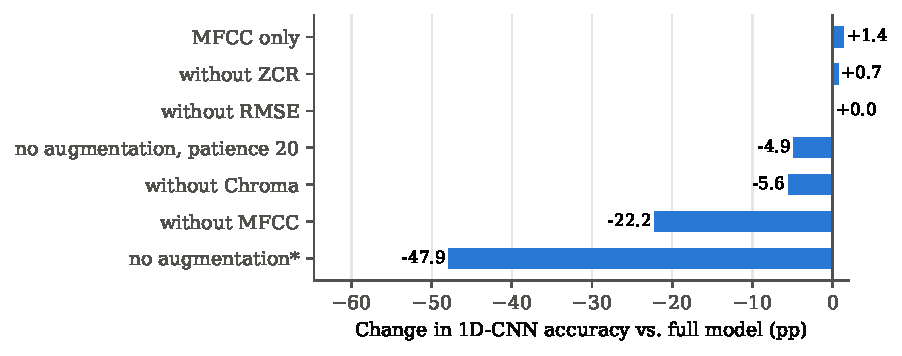
\includegraphics[width=\columnwidth]{../results/figures/fig_ablation.pdf}
\caption{Change in 1D-CNN accuracy when parts of the input are removed (paper-protocol split). *No augmentation
with the paper's early stopping, which halts before the model learns; see text.}
\label{fig:ablation}
\end{figure}


\subsection{Efficiency}
The 1D-CNN has \ParamsCnn{} parameters and the CNN\_Bi-LSTM \ParamsLstm{} (ensemble \ParamsEns{}). On a 4-core CPU,
training under the paper protocol took \FitMinCnn{} and \FitMinLstm{} minutes (\EpochsCnn{} and \EpochsLstm{}
epochs before early stopping), and inference costs \InferMsCnn{} and \InferMsLstm{} ms per clip. The SVM trains in
seconds and predicts in \InferMsSvm{} ms per clip, and it is only \PaperEnsOverSvm{} points behind the ensemble under the paper
protocol, which puts the value of the deep ensemble in perspective.

\section{Error Analysis and Discussion}
\label{sec:discussion}
\paragraph{Why the paper's protocol overestimates performance.} Emotion corpora such as RAVDESS contain a small
number of speakers who each record the same two sentences many times. A random split therefore places recordings of
the \emph{same actor saying the same sentence} in both training and test sets, and augmentation before the split
adds near-copies of the \emph{same recording}. Both violate the assumption that test data are independent of
training data. The 97\% figure measures recognition of familiar voices (or familiar recordings), not of emotion.

\paragraph{Why the models fail on new speakers.} The input is a globally standardised vector of absolute feature
values. MFCC and Chroma levels depend strongly on vocal-tract shape and fundamental frequency, i.e.\ on
\emph{who} is speaking; nothing in the pipeline removes speaker identity, so a model can reach high within-speaker
accuracy by learning speaker-specific baselines. For a new speaker those baselines are wrong. The dominant errors
(\ConfOne, \ConfTwo) are between low-arousal classes whose differences are subtle relative to between-speaker
variation. Merging RAVDESS \emph{calm} into \emph{neutral}, as the paper does, makes the neutral class more
heterogeneous and adds to this confusion.

\paragraph{Why women are recognised better.} We can only offer hypotheses: female voices typically have a higher and
wider pitch range, which Chroma and MFCC capture, so emotional pitch changes may be more separable; and the
augmentation (pitch shift of +0.7 semitones) never moves a voice across the male--female range. Speaker-level
normalisation or gender-balanced model selection would be the first mitigations to test.

\paragraph{Why cross-corpus transfer collapses.} Besides speakers, the corpora differ in utterance type (a full
sentence vs.\ ``Say the word \_\_''), duration (hence padding), speaker age and recording setup. The flattened,
position-dependent representation amplifies these differences: the same emotion expressed 0.3\,s later produces a
different input vector. The controlled padding check shows that one of these factors alone moves accuracy by
\OffsetGain{} points.

\paragraph{Take-away.} The paper's architecture is a reasonable lightweight model: it beats classical baselines under
every within-corpus protocol. But its reported accuracy is a property of the evaluation protocol as much as of the
model. For deployment, the speaker-independent figure (\AccSpkEns\%) and the cross-corpus figure (near chance)
are the relevant ones.


\section{Challenges Faced}
\begin{itemize}
  \item \textbf{Under-specified details.} The paper does not state whether augmentation precedes the split, how
        the ensemble is trained, or which label is used for RAVDESS \emph{calm}. We inferred the latter from its
        Table~1, trained the members separately and averaged them, and made the split order an explicit experiment (P2).
  \item \textbf{Inconsistent parameter table.} The paper's Table~2 lists 6,176 parameters for the last
        convolution, which does not match a 128-channel Bi-LSTM output; we followed the layer description.
  \item \textbf{Compute.} Convolving a 3,672-step input with 128 filters is expensive on a CPU: one epoch takes
        about 30\,s for the 1D-CNN and longer for the Bi-LSTM variant, so the \NumTrainings{} training runs of this
        study took roughly \ComputeHours{} hours. We therefore ran the ablation on one split rather than four folds.
  \item \textbf{Dataset access and duplicates.} Both Kaggle datasets ship duplicated folders; without
        de-duplication identical files would appear in both training and test sets.
  \item \textbf{Different clip lengths.} TESS clips are about 2\,s long, so after the paper's 0.6\,s offset
        \TessPadPct\% of TESS frames are zero padding versus none for RAVDESS, an input shift that matters for
        cross-dataset transfer (Sec.~\ref{sec:discussion}).
\end{itemize}

\section{Limitations and Future Work}
Both corpora contain acted, scripted North-American English speech, so even our strictest protocols overestimate
performance on spontaneous speech. TESS has only two female speakers, so the reverse cross-dataset direction trains
on two voices, and the gender analysis is restricted to RAVDESS. We used one random seed per configuration; fold-level
standard deviations indicate variance across speakers but not across initialisations. Natural next steps are
speaker-level feature normalisation, domain-adversarial training, multi-corpus training, and adding CREMA-D
(91 speakers) to test transfer to a larger, more diverse corpus.

\section{Conclusion}
We re-implemented a recent lightweight SER ensemble and asked how far its near-perfect accuracy generalises. Five
findings stand out. (1) Under a leak-free random split our implementation reaches \AccPaperEns\%, not 97.57\%.
(2) Applying augmentation before splitting reproduces the reported level (\AccLeakyEns\%) because almost every test
sample has a near-copy in training. (3) For unseen speakers accuracy drops to \AccSpkEns\%, still well above
classical baselines. (4) Across corpora the model is near chance, partly because the paper's fixed offset leaves
\OffsetPadPaper\% of TESS frames as zero padding. (5) The model is significantly less accurate for male speakers
(\GenderGapEns{} points). For practitioners the lesson is concrete: report speaker-independent and cross-corpus
results, split before augmenting, and check performance per demographic group before deploying an emotion
recogniser.


\paragraph{Reproducibility.} All code, the exact library versions and the scripts that generate every number and
figure in this report are in the project repository (\texttt{README.md}); the pipeline runs end-to-end with four
commands.


\small
\bibliographystyle{unsrtnat}
\bibliography{refs}

\end{document}
